\chapter{Introduction}

Randomisation is essential to research areas such as \textit{probabilistic programming},~dependability (system components with uncertainty),~distributed computing (symmetry breaking),~and planning (unknown and noisy environments).
Probabilistic programs are powerful modelling apparatus of systems containing probabilistic uncertainty.
Systems with unreliable and unpredictable behaviour require the~use of such a~mathematical apparatus established on probability theory.
Designing such systems exhibiting a~desirable behaviour \,--\, e.g. selecting the~optimal power management strategy or a~network protocol increasing the~packet throughput \,--\, is challenging for reasoning over multiple alternative designs.
Their applications cover a~broad range of research areas,~including,~e.g. analysis of (quantitative) software product lines~\cite{spl1,spl2},~strategy synthesis in planning under partial observability~\cite{pomdp1,pomdp2},~or design of communication protocols~\cite{herman1,herman2}.

A~set of declarative temporal constraints often expresses the~efficiency and correctness of the~probabilistic programs.
The~model checkers for probabilistic systems,~such as \storm{}~\cite{STORM} or \prism{}~\cite{KNP11},~provide automated verification of such constraints.
However,~these probabilistic model checkers require a~fixed model or a~fixed program,~contrary to their usage requirements when modelling probabilistic programs.
Developers need to verify the~system designs as early as possible at the~developing process to maintain its costs tractable and as best as possible.
System designs are prevailingly incomplete at the~initial development phases because,~in most cases,~there are no known all system specifications or intentionally left out potentially.
These undefined system specifications are called \textit{holes},~and they can,~e.g.,~reflect an~unspecified component for wireless specification or a~partially implemented controller.
The~synthesis's primary purpose is through analysis reveals a~concrete subsystem with fully-defined behaviour and eventually reveals optimal designs when they are requested.
A~vital aspect of the design cycle is design space explorations,~i.e. exploring all possible designs.
When considering a~Markov chain (MC) as the~mathematical apparatus of a~probabilistic program,~then the~design space represents a~family of such chains,~and the~synthesis task is to find the~one that satisfies a~given specifications.

A~\textit{one-by-one} approach can naively solve the~synthesis problem by analysing all unique designs~\cite{spl3,onebyone}.
On the contrary,~the whole design space can also be modelled as a~single \textit{all-in-one} Markov decision process~\cite{spl3,allinone}.
However,~enumerating all members of design space (realisations) is unfeasible due to its combinatorial explosion, and the size of such all-in-one MDP is proportional to the number of candidate designs.
Unfortunately,~the~double state-space explosion problem renders both of these approaches infeasible for large families.
Other approaches consider evolutionary search algorithms for the~synthesis of software systems~\cite{spl2}.
These methods remain incomplete and cannot efficiently solve more challenging systems,~e.g.,~which design satisfies the specification \textit{optimally}.

In this work,~we will focus on a~complete state-of-the-art approach for the~synthesis of probabilistic programs.
This approach was first introduced in \textit{Andriushchenko} master’s thesis~\cite{roman-DP}, followed~by its improvement in~\cite{tacas21}.
It combines two sophisticated methods providing an~analysis of whole design sub-families at once.
The~first method analyses each design from a~given sub-family individually and constructs critical sub-systems of counter-examples to prune all designs behaving incorrectly \,--\, the~so-called \textit{counter-example guided inductive synthesis} (CEGIS)~\cite{cegis}.
The~second method,~called abstraction refinement (AR)~\cite{cegar},~immediately analyses the~entire design space and refines it into design sub-families when the~analysis yields inconclusive results.
Both of these methods have shown convincing results,~although each faces certain limitations.
They are incomparable because one method can be more suitable for specific probabilistic programs classes and conversely.
The~approach presented in this work integrates both these methods and it manages to significantly outperform them,~sometimes by a~margin of orders of magnitude.

All these presented methods consider \textit{topology synthesis} task assuming a~finite set of parameters that affect the~model topology,~where the~individual parameters represent the~undefined system specifications.
This task focuses on Markov chains families having different topologies of the~state space and,~as a~consequence,~different sets of reachable states.
However,~another area of synthesis tasks considers a~Markov chain with fixed topology but undefined transition probabilities.
This area has been discussed by approaches of model repairing~\cite{model-repair-1,pathak-et-al-nfm-2015} and techniques for \textit{parameter synthesis}~\cite{ceska2014robustness,Quatmann2016}.
When modelling real-world systems,~combining the two tasks can quickly occur,~but the~support to solve such a~\textit{combined synthesis} task does not exist.

\subsubsection*{Key Contributions.}
This thesis considers a~novel integrated method introduced in the~previous works~\cite{roman-DP,tacas21} as a~base stone.
Initially,~this method was designed only for feasibility synthesis task with one specification.
However,~probabilistic programs often have to satisfy specifications expressed as a~conjunction of several temporal logic constraints.
Therefore, we designed an~extension of this method to support \textit{multi-property specifications} and \textit{optimal synthesis} task.
The~designed extension for multi-properties is performed in the~same loop as the~origin single-property synthesis, with~necessary modifications: \textit{AR} need to analyse satisfiable specifications within inference sub-families no longer,~and \textit{CEGIS} analyses each specification individually and constructs counter-examples whenever a~given specification is unsatisfiable.
Consequently,~the~novel integrated method inherits the~benefits of \textit{AR} and \textit{CEGIS} in its favour also at multi-property synthesis.
\textit{Optimal synthesis} is a~particular instance of \textit{multi-property synthesis},~and it can find an application in various domains.
In particular,~specification set includes so-called violation property representing the currently optimal solution,~and its threshold is updated whenever a~new optimal solution is found.
Moreover,~we designed support for the~relaxed variant of the~optimal synthesis,~so-called $\varepsilon$-optimal synthesis,~which is in most cases even faster.
We evaluate designed extensions on an~extensive set of real-world case studies. 
We confirm the~results of a~novel approach presented in the~previous works and found the~following conclusions relating to these extensions.
A~novel integrated method is orders of magnitude faster than one-by-one enumeration when analysing the~single property.
A~multi-property synthesis slows down both approaches,~although the~novel method slow down is almost negligible.
An~optimal synthesis slows down only the~integrated approach,~yet it is still incomparably faster than enumeration.
The~assumption that $\varepsilon$-optimal synthesis can significantly speed up the~whole optimal synthesis process was also confirmed.

\todo{Parameter synthesis ...}


\subsubsection*{Structure of this paper.}
In Chapter~\ref{chap:synthesis},~we formulate a~probabilistic synthesis problem and introduce a~state-of-the-art novel integrated method based on two modern approaches \textit{CEGIS} and \textit{AR}.
Chapter~\ref{chap:advanced} develops vital ideas associated with integrating the \textit{multi-property} synthesis and \textit{optimal} synthesis within the presented integrated method.
Then, in Chapter~\ref{chap:combined}, we develop critical ideas associated with integrating the combined synthesis \,--\, consists of topology and parameter synthesis \,--\, within the considered method.
Chapter~\ref{chap:paynt} introduces a~new tool called \toolname{} and its architecture,~which implemented the~presented methods.
Chapter~\ref{chap:experiments} evaluates our solutions on a~broad range set of real-world case studies and compares them with the~baseline enumeration approach.
Finally,~Chapter~\ref{chap:conclusion} closes this thesis with the~notes
and issues that can serve as a~baseline point for the~follow-up research and potential improvement of designed solutions.

\chapter{Synthesis of Probabilistic Programs}\label{chap:synthesis}

\section{Problem Statement}
This section formalises necessary ingredients and the~problem statement for probabilistic synthesis.
We introduce definitions that assume parameters affecting MCs' topology,~and their adjustable versions for parameter synthesis we will introduce in Section~\ref{chap:combined}.
The following definitions are taken from the existing sources, mainly from~\cite{roman-DP,tacas21}, where a more detailed description can also be found.

\subsection{Markov Chains}

\begin{definition}[Distribution]
\cite{tacas21} 
    A \textit{discrete} distribution over a~finite or countably infinite set $X$ is a~function $\mu: X \rightarrow [0,1]$ s.t. $\sum_{x \in X} \mu(x) = \mu(X) = 1$.
    The~set of all distributions on $X$ is denoted $Distr(X)$.
    The support of a distribution $\mu$ is $supp(\mu) = \{ x \in X \lvert \mu(x) > 0 \}$.
    % A distribution is \textit{Dirac} if $\lvert supp(\mu) \rvert = 1$.
\end{definition}

\begin{example}
    Let $X = \{x_0, x_1, x_0\}$ be a finite set.
    Let function $\mu: X \rightarrow [0,1]$ defined as $\mu: [x_0 \mapsto \frac{1}{2}, x_1 \mapsto 0, x_2 \mapsto \frac{1}{2}]$ be a \textit{probability distribution} on $X$, i.e. $\mu \in Distr(X)$.
    The support of $\mu$ is $supp(\mu) = \{x_0, x_2 \}$, and for simplification, we writes such distributions as $\mu = \frac{1}{2} : x_0 + \frac{1}{2} : x_2$.
\end{example}


\begin{definition}[MC]
\cite{tacas21}
    A Markov chain (MC) D is a~triple $\mc$,~where $S$ is a~finite set of states,~$s_0 \in S$ is an~initial state,~and $\mathbf{P}: S \rightarrow Distr(S)$ is a~transition probability matrix.
    We write $\mathbf{P}(s, t)$ to denote $\mathbf{P}(s)(t)$.
    The state $s$ is \textit{absorbing} if $\mathbf{P}(s, s) = 1$.
\end{definition}

Instinctively,~we can imagine an~$MC$ as a~state-transition system with the~following semantics.
A~probability distribution for each state $\forall s \in S: \mathbf{P}(S)$ represents a~stochastic choice of firing the~transition from such state $s \in S$ to one of its successors states $s' \in supp(\mathbf{P(S)})$.
Consequently,~an~$MC$ defined with such semantics has a~\textit{Markov property} (memorylessness), which is essential when modelling systems and efficient analysis.
This property declares that the~probability of the~transition from state $s \in S$ to state $s' \in supp(\mathbf{P(S)})$ depends only on the~current state,~and it is independent of the~taken path of chain to state $s$.
We can see that each state of an $MC$ disposes of a unique probability distribution over its possible successor states.
In the~following definition,~we define an~extension of $MCs$ introducing a~non-deterministic choice between several probability distributions over each state.

\begin{definition}[MDP]
\cite{roman-DP}
    A Markov decision process (MDP) $M$ is a~quadruple $\mdp$ ~where $S$ is a~finite set of states,~$s_0 \in S$ is an~initial state,~$Act$ is a~finite set of actions,~and $\mathbb{P}: S \times Act  \nrightarrow Distr(S)$ represents a~(partial) transition probability function. 
\end{definition}

When an~$MDP$ is currently in the~state $s \in S$,~it has a~non-deterministic choice of an action $a \in Act(s)$ leading to the~one possible probability distribution $P(s)(a)$ over its successors' states.
These actions cause the~non-deterministic behaviour of an~$MDP$.
Still,~this property can be suppressed by applying a~\textit{scheduler},~which selects one specific action in each state,~i.e.,~transforms an~$MDP$ to an~$MC$.
For more material about schedulers and other details about Markov chains,~see~\cite{roman-DP}.

\subsection{Families of Markov Chains}
This thesis considers a~parametric transition probability function as an~explicit representation of an~MCs family.
Such explicit representation relieves the~presentation and provides to describe exciting and practical problems for probabilistic synthesis.
On the~other hand,~arbitrary probabilistic programs permit the~modelling of more complex and independent parameter structures~\cite{cegar}.
In this thesis and our implementation,~we consider a~more flexible high-level modelling language,~see Section~\todo{?}.

\begin{definition}[Family of MCs]
\cite{cegar}
    A~\emph{family of MCs} $\fml$ is a~quadruple $\family$  where $S$ is a~finite set of \emph{states}, $\sinit \in S$ is an~\emph{initial state},~$K$ is a~finite set of parameters with domains $T_k \subseteq S$ for each $k \in K$,~and $\fpm : S \rightarrow Distr(K)$ is a~family of transition probability functions.
\end{definition}

The~transition probability function $\fpm$ of MCs family $\fml$ maps each state $s \in S$ to the~probability distribution over parameters from $K$.
As we mentioned above,~these parameters represent undefined system specifications when the~probabilistic synthesis is considered.
This function $\fpm$ yields a~specific MC when we instantiate each parameter $k \in K$ with the~specific value from its domain $T_k \subseteq S$.
We call such instantiated MC as \textit{realisation},~and the~following definition describes it.

\begin{definition}[Realisation]
\cite{cegar}
A~\emph{realization} of a~family $\fml = \family$ of MCs is a~function $r: K \rightarrow S$ s.t.~$\forall k \in K :  r(k) \in T_k$. 
A~realization~$r$ yields a MC $\fmlr = (S,\sinit,\fpm(r))$,~where $\fpm(r)$ represents the~transition probability matrix where each parameter $k \in K$ is substituted with $r(k)$. 
Let $\rlzf$ denote the~set of all realisations for $\fml$.
\end{definition}

A~set $\prod_{k \in K} T_k$ representing all possible parameter combinations values has the~same semantics as a~set $\rlzf$ representing all family realisations.
In other words,~we can define the~\textit{size of the family} of MCs in the~following way: $\lvert \fml \rvert := \lvert \prod_{k \in K} T_k \rvert = \lvert \rlzf \rvert = \prod_{k \in K} \lvert T_k \rvert$.
The~family size $\lvert \fml \rvert$ is finite because of the~finiteness of each parameter domain $T_k \subseteq S$,~but it is exponential in the~number of parameters $\lvert K \rvert$.
We note $\rlz$ as the~sub-families induced from the~whole family $\rlzf$.
The~individual MCs within the~family share the~same state space $S$,~but their set of reachable states can vary.

\begin{example}[Family of MCs]\label{exam:mcfamily}
Let $\fml = \family$ be a~family of MCs,~where $S = \{s_0, s_1, s_2, s_3\}$ and $K = \{ k_0, k_1\}$ with domains $T_{k_0} = \{s_0, s_2\}$,~and $T_{k_1} = \{s_1, s_3\}$.
The parametric transition function $\fpm$ is defined as follows:
\begin{align*}
    \fpm(s_0) &= 0.5 : k_0 + 0.5 : k_1  &  \fpm(s_1)  &= 0.5 : k_1  + 0.5 : k_0 \\
    \fpm(s_2) &= 1.0: k_1   &  \fpm(s_3)  &= 1.0 : s_3
\end{align*}
Figure~\ref{fig:mcfamily} draws the~MCs family $\fml$ that correspond to all possible realisations: $\lvert T_{k_0} \rvert \cdot \lvert T_{k_1} \rvert = 2 \cdot 2 = 4$.
We note that these MCs have a~different topology of the~underlying state space,~resulting in different sets of reachable states.
\end{example}

\begin{figure}[ht!]
\centering
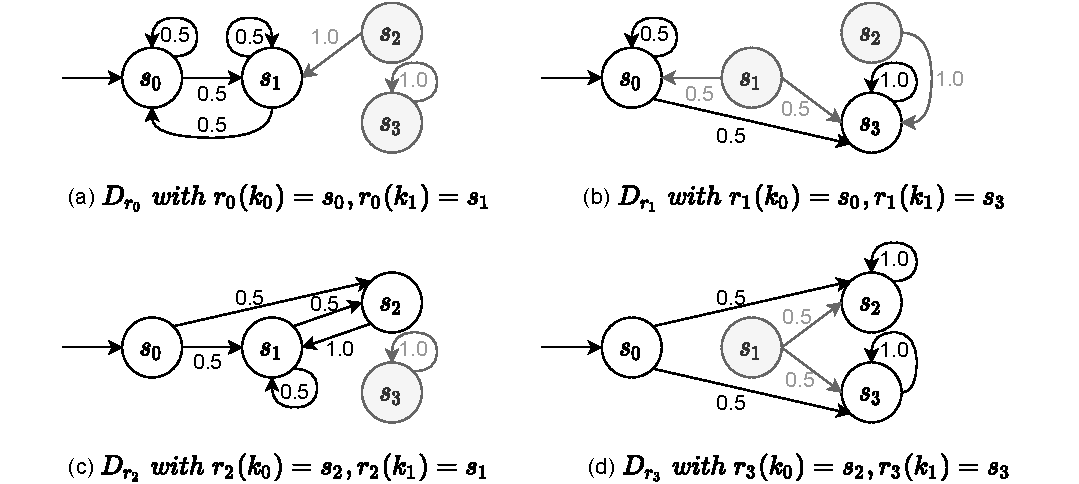
\includegraphics[width=0.9\textwidth]{figures/MCFamily.pdf}
\caption{A family $\fml$ of four various realisations. Unreachable states are greyed out.}%
\label{fig:mcfamily}%
\end{figure}

\subsection{Probabilistic Synthesis}

\begin{definition}[Specification]
In our work,~we focus on the~conjunctions of specifications with \textit{reachability} and \textit{expected rewards}.
Let $T$ be a~set of target states,~then the~reachability property $\varphi \equiv \reachability{\bowtie}{\lambda}{T}$ where $\bowtie \in \{<, \leq, >, \geq\}$ and $0 \leq \lambda \leq 1$ expresses that the~probability of reaching $T$ refers to $\lambda \in [0,1]$ in agreement with $\bowtie$.
Expected reward property $\phi \equiv \reward {\bowtie}{\lambda}{T}$ expresses that the~expected reward accumulated before $T$ is reached refers to $\lambda \in \mathbb{R}^+$ in accordance with $\bowtie \, \in \{<, \leq \}$.
Let $\mathcal{P}[r]$ be a~program induced by the~realisation $r$,~we denote $\mathcal{P}[r] \models \varphi$ when this program satisfies the~specification $\varphi$.
Let $\varPhi = \{ \varphi_i \}_{i \in I}$ be a~finite set of specifications,~when $\forall i \in I: \mathcal{P}[r] \models \varphi_i$ then we write $\mathcal{P}[r] \models \varPhi$.
\end{definition}

We aim to two kinds of synthesis tasks for a~given probabilistic program described with a~realisation set $\rlzf$,~and a~specification set $\varPhi$.
The first task tries to identify just one realisation $r \in \rlzf$ that satisfy the~given specification set $\varPhi$.
This task represents a~special instance of the~threshold synthesis,~which tries to divide the~realisation set $\rlzf$ into two subsets based on their satisfiability.
We do not address this synthesis task in our work.
The second task on which we focus our attention is finding a~realisation that minimises or maximises a~given objective.

\begin{definition}[Feasibility]
Find a realisation $r \in \rlzf$ such that $\mathcal{P}[r] \models \varPhi$. 
\end{definition}

\begin{definition}[Minimality]
For property $\phi_{\max}$, find a realisation $r^* \in \rlzf$ such that:
$$r^* \in \argmax_{r \in \rlzf} \left \{ \prob[\sketch[r] \models \phi_{\max}] \mid \sketch[r] \models \varPhi \right \}.$$.
\end{definition}

We defined only minimal synthesis task for probability property,~but its variants for maximisation and expected rewards may be defined analogously.
Moreover, we focus also to a relaxed variant of minimal synthesis, the so-called \textit{$\varepsilon$-minimal synthesis}, defined as follows: $\mathcal{P}[r^*] \models \varPhi \; and \; 
\mathbb{P}[\mathcal{P}[r^*] \models \varphi_{min}] \leq (1 - \varepsilon) \cdot \min_{r \in \mathcal{\overline{R}}} \{ \mathbb{P}[\mathcal{P}[r] \models \varphi_{min}] \; \lvert \; \mathcal{P}[r] \models \varPhi \}.$

\begin{example} (Synthesis problems)
Assume an~MCs family $\fml$ from Example~\ref{exam:mcfamily} and the specification $\phi = \reachability{\geq}{0.1}{\{s_1\}}$.
The solution to the~feasibility synthesis problem is,~for example,~the~realisation $r_0$, since $D_{r_0}$ has a~probability of $\frac{2}{3}$ to reach state $s_1$.
For $\varPhi = [F \; \{s1\}]$,~the~solution to the~maximal synthesis problem on MCs family $\fml$ is the~realisation $r_2$,~as MC $D_{r_2}$ has a~probability equal to one to reach state $s_1$.
\end{example}

\section{Synthesis Methods}
Existing methods for a~probabilistic programs synthesis can be separated into two orthogonal classes.
The~first class involves complete methods that prove the~non-existence,~or potentially optimally,~of the~given probabilistic program.
On the~contrary,~incomplete methods handling various evolutionary techniques and intelligent search strategies form the~second one~\cite{spl2}.
However,~these incomplete methods cannot treat unfeasible and optimal synthesis problems compared to the~complete methods.
Therefore, we focus on the~complete state-of-the-art methods even though the~incomplete methods provide a~valuable flexibility level.
As a~reference and baseline method,~we consider a~\textit{one-by-one} approach that enumerates through each design space member~\cite{onebyone}.
An~explosion of the~design space renders this technique unfeasible for large families,~necessitating using advanced approaches utilising the~arbitrary structure of~the Markov chain family.

This thesis focuses on the~complete methods considered within the~\textit{oracle-guided} synthesis approach~\cite{oracle1,oracle2}.
The~control unit called \textit{learner} selects a~realisation $r$ from the~designs family and passes it to the~performing unit called \textit{oracle}.
This unit provides an~answer to whether realisation $r$ satisfies a given specification $\varPhi$.
Whenever it is not this case,~it provides supplementary information representing counterexample (CEGIS) or bounds from MC model checking (AR).
For purposes of this thesis, two various orthogonal oracles can be considered:
\begin{enumerate}[label=(\roman*)]
    \item \textbf{Inductive Oracle} (CE): It tries to infer the~declarations (counter-examples) about other family members by analysing individual realisation~\cite{cegis}.
    \item \textbf{Deductive Oracle} (AR): Abstraction refinement oracle considers more family members at once and then infers the consequences of these members' constructed aggregation~\cite{cegar}.
\end{enumerate}
The~novel integrated approach,~the~so-called \textit{hybrid} method,~combines both these oracles and can thus take advantage of the~benefits offered by both approaches~\cite{roman-DP,tacas21}.
We illustrate the~cooperation between the~individual units within this method in Figure~\ref{fig:adaptivesynt}.
The~learner unit maintains the~subfamilies queue $\rlz' \subseteq \rlzf$ for subsequent processing and decides which oracle is selected based on their previous efficiency.
The~\textit{CE-Oracle} analyses the~family member $r$ and,~when it satisfies the~given specification $\varPhi$,~then returns it as a~solution.
On the~other hand,~it can generalise the~analysed realisation $r$ into a~subfamily $\rlz'$,~and the~learner unit can discard it from the~whole design space $\rlzf$.
Moreover,~this oracle exploits the~MDP bounds when constructing counterexamples,~thanks to which it can generate more petite generalisations.
The~\textit{Abstr-Oracle} analyses a~given sub-family $\rlz \subseteq \rlzf$,~and according to the~result,~it performs the~subsequent action.
When all realisations $r \in \rlz$ satisfy $\varPhi$,~then it returns the~overall synthesis result as feasible.
In another case,~when all realisations violate $\varPhi$,~the~whole analysed sub-family $\rlz$ will be discarded from the~families queue $\rlzf$ by the~learner.
The last option returns safe bounds on the best- and worst-case behaviour of all realisations in $\rlz$ considered $\varPhi$ when the analysis result is inconclusive.

\begin{figure}[ht!]
    \centering
     \begin{tikzpicture}
    \node[rectangle, draw, inner sep=8pt] (learner) {Learner};
    \node[rectangle, draw, inner sep=8pt,right=2.7cm of learner] (oracle) {CE-Oracle};
       \node[rectangle, draw, inner sep=8pt,left=2.7cm of learner] (abst) {Abstr-Oracle};
    \node[above=0.5cm of learner] (rlz) {$\rlzf$};
    \draw[->] (rlz) -- (learner);
    \node[above=0.5cm of oracle] (phi) {$\varPhi$};
    \draw[->] (phi) -- (oracle);
    \node[above=0.5cm of abst] (phiab) {$\varPhi$};
    \draw[->] (phiab) -- (abst);
    \draw[->] (learner) edge[bend left=10] node[above] {\scriptsize{$r \in \rlzf$}+bounds} (oracle);
    \draw[->] (oracle) edge[bend left=10] node[below] {\scriptsize{$\rlz' \subseteq \rlzf$ violate $\varPhi$}} (learner);
      \draw[->] (learner) edge[bend right=10] node[above] {\scriptsize{$\rlz \subseteq \rlzf$}} (abst);
    \draw[->] (abst) edge[bend right=10] node[below,align=center] {\scriptsize{bounds \emph{or} $\rlz$ violates}} (learner);
    
    \node[below=0.4cm of oracle] (sat) {$r \models \varPhi$};
    \draw[->] (oracle) -- (sat);
    \node[below=0.4cm of abst] (allsat) {each $r \in \rlz$, $r \models \varPhi$};
    \draw[->] (abst) -- (allsat);
    \node[below=0.4cm of learner] (unsat) {no $r \models \varPhi$};
    \draw[->] (learner) -- (unsat);
    \end{tikzpicture}
  \vspace{-0,5em}
    \caption{Oracle-guided synthesis (adapted from~\cite{tacas21}).}
    \label{fig:adaptivesynt}.
    \vspace{-1em}
\end{figure}

\paragraph{Hybrid Method.}
An~extended synthesis approach was introduced in~\cite{roman-DP,tacas21} using the~abstraction refinement to family prune and accelerating the~construction of counter-examples by CE-oracle.
Its main idea is to perform a~limited number of abstraction refinement loops and then invoke CEGIS to one of the~refined sub-families.
It turned out that a~moment of the~switching can be crucial,~and therefore,~the~method has to detect the~rightest moment.
One AR iteration is typically significantly slower than one CEGIS iteration since the~AR iteration involves an~MDP model-checking,~which inspires whole method workflow.
The~advance of the~hybrid methods is also constructing counter-examples within the~CEGIS loop,~where it uses a~fast greedy approach providing smaller generalisations.

\begin{algorithm}[H]
\hspace*{\algorithmicindent} \textbf{Input:} A MCs family $\fml$, a reachability property $\varphi$. \\
\hspace*{\algorithmicindent} \textbf{Output:} $Realization\; r \in \rlzf \; s.t. \; \mathcal{D}_r \models \varphi$, otherwise UNSAT. \\
\vspace*{-1.5em}
\begin{algorithmic}[1]
    \STATE $\rlzf \leftarrow \{ \rlz^{\fml} \}$ \hfill \textbf{// each analysed (sub)-family also holds bounds}
    \STATE $\delta_{CEGIS} \leftarrow 1$ \hfill \textbf{// time allocation factor for CEGIS}
    \WHILE{$\rlzf \neq \emptyset$}
        \STATE result, $\rlzf'$, $\sigma_{AR}$, $t_{AR}$ $\leftarrow$ AR($\rlzf$, $\varphi$)
        \IF{\textbf{satisfiable}(result)}
            \RETURN result
        \ELSE
            \STATE result, $\rlzf''$, $\sigma_{CEGIS}$ $\leftarrow$ CEGIS($\rlzf'$, $\varphi$)
            \IF{\textbf{satisfiable}(result)}
                \RETURN result
            \ELSE
                \STATE $\delta_{CEGIS}$ $\leftarrow$ $\sigma_{CEGIS}$ / $\sigma_{AR}$
                \STATE $\rlzf$ $\leftarrow$ $\rlzf''$
            \ENDIF
        \ENDIF
    \ENDWHILE
    \RETURN{UNSAT}
\end{algorithmic}
\caption{Hybrid method: Feasibility synthesis with single property.}
\label{alg:hybrid}
\end{algorithm}

As we said above,~this \textit{novel integrated} method combines inductive and deductive oracles,~and we briefly summarise their operation.
CEGIS iterates through all family members (realisations) until it reached the~satisfying realisation,~if such exists,~or when it explores the~whole design space.
Moreover,~it constructs counter-examples whenever the~analysed realisation $r \in \fmlr$ unsatisfying the~given specification $\varPhi$.
Realisations subset $\rlz' \subseteq \rlzf$ represents such counter-examples that CEGIS subsequently prunes from the~analysed design space $\rlzf$.
On the~other hand,~an AR loop builds MDP models from the~sub-families queue $\rlz \subseteq \rlzf$ that model-checkers analyse in follows.
When the~analysis results are inconclusive,~an AR refines the~analysed sub-family and  stores the~obtained satisfiability bounds for further processing within CEGIS loop.
Method allocates the~time per both loop according to their performance,~e.g.,~it can consider the~number of pruned MCs per timed unit and estimates an~efficiency from it.
Namely,~when it notices that AR prunes sub-families twice as slow as CEGIS,~it increases time twice in the~next round for CEGIS.
The resulting algorithm is summarised in Algorithm~\ref{alg:hybrid},~adapted from~\cite{tacas21}.


\chapter{Advanced Methods for Probabilistic Synthesis}\label{chap:advanced}


\chapter{Combined Probabilistic Synthesis}\label{chap:combined}


\chapter{Tool Architecture}\label{chap:paynt}


\chapter{Experimental Evaluation}\label{chap:experiments}


\chapter{Final Considerations}\label{chap:conclusion}


\section{Future Research}
\section{Conclusions}